\documentclass{resume}

\begin{document}

\fontfamily{phv}\selectfont

\noindent
\begin{tabularx}{\linewidth}{@{}m{0.5\textwidth} m{0.5\textwidth}@{}}
{
    \Large{Dawid Bińkuś} \newline
    \small{
        \clinksecond{
            \faEnvelope\ \href{mailto:dawid.binkus0@gmail.com}{dawid.binkus0@gmail.com}
            \newline
            {\fontdimen2\font=0.75ex \faPhone\  +48516126394} 
            \newline
            \faGithub\ \href{https://github.com/inql}{github.com/inql}
            \newline
            \faLinkedin\ \href{https://www.linkedin.com/in/dawid-binkus/}{linkedin.com/in/dawid-binkus/}
        } \newline
        \faHome\ Gdańsk, Poland
    }
} & 
{
    \begin{center}
    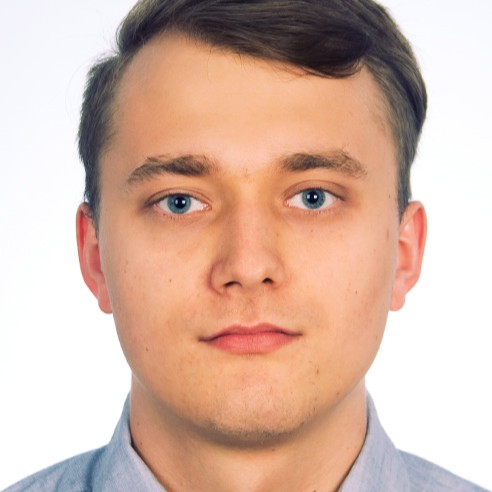
\includegraphics[width=3cm]{images/photo.jpeg}
    \end{center}
}
\end{tabularx}
\begin{center}
\begin{tabularx}{\linewidth}{@{}*{2}{X}@{}}
% left side %
{
    \csection{EXPERIENCE}{\small
        \begin{itemize}
            % item 1 %
            \item \frcontent{Intel Technology Poland}{Deep Learning Software Engineer}{
                Designing and delivering solutions for VPU processors (C++).
                Developing software stack, bug fixing.
                Maintaining development enviroments with containerization.
                Backup Scrum Master for development team.
            }{July 2020 onwards}
            % item 2 %
            \item \frcontent{Intel Technology Poland}{Software Validation Engineer}{
                Implementer of automation for functional tests for Cable Modems (Java, jUnit based framework).
                \newline
                Creating and maintaining test setups, supporting developers with debugging of new features.
            }{May 2019 to June 2020}
            % item 2 %
            \item \frcontent{Intel Technology Poland}{Software Validation Intern}{
                Responsible for defining and automating functional/performance validation cases for DOCSIS modems.
                }{July 2018 to May 2019}
        \end{itemize}
    }
    \csection{EDUCATION}{\small
        \begin{itemize}
            % item 1 %
            \item \frcontent{M.S. Computer Science}{University of Gdańsk}{}{2021}
            \item \frcontent{B.S. Computer Science}{University of Gdańsk}{}{2019}
        \end{itemize}
    }
} 
% end left side %
& 
% right side %
{
    \csection{SKILLS}{\small
        \begin{itemize}
            \item \textbf{Technologies} \newline
            {\footnotesize C++, Python, Java, Scala, Bash, Docker, Linux}{}{}
            \item \textbf{Patterns \& Practices} \newline
            {\footnotesize Object Oriented Programming, Functional Programming, CI \& CD}
            \item \textbf{Project Management} \newline
            {\footnotesize Agile, Scrum}
            \item \textbf{Others} \newline
            {\footnotesize TCP/IP, Networking protocols, Wireshark}
        \end{itemize}
    }
    \csection{PROJECTS \& ACHIEVEMENTS}{\small
        \begin{itemize}
            \item \frcontentprojects{OnePass \clink{\href{https://github.com/inql/OnePass}{[github.com/inql/OnePass]}}}{CLI tool for storing passwords}{}{C++, Boost, CryptoPP}
            \item \frcontentprojects{StartOwl \clink{\href{https://github.com/inql/StartOwl}{[github.com/inql/StartOwl]}}}{News aggregator based on RSS and Allegro API}{}{Scala, Akka}
            \item \frcontentprojects{AlgorIT \clink{\href{https://mat2tab.ug.edu.pl/}{[Mat2Tab]}}}{3rd place in nationwide competiton Mat2Tab 2017 - for application which helps to resolve flowcharts algorithms}{}{GameMaker}
        \end{itemize}
    }
    \csection{OTHER HIGHLIGHTS}{\small
        \begin{itemize}
            \item {\footnotesize Completed \textbf{Advanced Modern C++} course provided by \textit{\clinksecond{\href{https://train-it.eu/}{train-it.eu.}}}}
        \end{itemize}
    }
    \csection{HOBBIES \& INTERESTS}{\small
        \begin{itemize}
            \item {\footnotesize Open Source}
            \item {\footnotesize Board \& Video Games}
            \item {\footnotesize IoT}
        \end{itemize}
    }
}
\end{tabularx}
\end{center}
\end{document}